\documentclass[twocolumn, groupedaddress]{revtex4-1}
\usepackage[utf8]{inputenc}
\usepackage{amsmath}
\usepackage{amsfonts}
\usepackage{amssymb}
\usepackage{graphicx}											% Use pdf, png, jpg, or eps§ with pdflatex; use eps in DVI
\usepackage[left=2cm, right=2cm, top=2cm, bottom=2cm]{geometry}
\usepackage{float}												% for controlling the position of objects ie. tables

\usepackage[small, bf]{caption}									%Adjust caption size of figures, tables, pictures...
\setlength{\captionmargin}{15pt}
										
\graphicspath{{images/}}											% folder where images are stored in current directory


% --------------------------- Code for placing two figure side by side ------------------------------------------------------------------
\usepackage{caption}
\usepackage{subcaption}

% --------------------------- Code for the bibliography ---------------------------------------------------------------------------------
\usepackage{natbib}												% For fancy in-text citations
\bibliographystyle{plain}



\begin{document}

\author{Curtis Rau}
\author{Colin Gordon}
\author{David Witalka}
\author{Samuel Akwei-Sekyere}
\affiliation{Michigan State University}
\title{A Search Algorithm for Continuous Phase Modulated Gravitational Waves Originating from Binary Neutron Star Systems}

\begin{abstract}
-we are given time series data.
-we are looking for phase modulated gravitational waves.
-form of phase modulation depends on the nature of the binary orbit.
\citep{Saulson}
\citep{LSCall}
\citep{Deanna}
\citep{folland}
\citep{griffiths}
\end{abstract}

\maketitle



\section{Introduction (Curtis Rau will be doing this)}

Just last week the discovery of gravitational waves was announced.  We have reason to believe the most numerous sources of gravitational waves in the universe are neurton stars.  These stars are expected to emmit single frequency waves over very long periods of time.  It is also believed that roughly half of all neutron stars are in binary systems, ie. two of them orbiting around eachother.  This phase modulates the signal which has the effect of reducing the power in the carrier frequency and distributes it into higher and lower harmonics.  This spreads out the power of the signal over a range of frequencies which makes it harder to detect these waves.  Especially because there is a high noise to signal ratio in the LIGO data.  It would be nice to have an algorithm that does the following:

\begin{equation}
G e^{i\left( \omega_c t + \Gamma \cos (\Omega t + \phi ) \right)} \to G \delta (\omega_c) \delta (\Gamma ) \delta (\Omega )
\end{equation}

Previous methods have utilized, where f(t) is the data.

\begin{align}
G e^{i\left( \omega_c t + \Gamma \cos (\Omega t + \phi ) \right)} &= f(t) \\
G e^{i\omega_c t} &= f(t) e^{-i\Gamma \cos (\Omega t + \phi)}			 \\
F_t \left[ G e^{i\omega_c t} \right] &= F_t \left[ f(t) e^{-i\Gamma \cos (\Omega t + \phi)} \right]
\end{align}

invoking the convolution theorem

\begin{equation}
\frac{G}{\sqrt{2\pi}} \delta (\omega_c - \omega) = F_t \left[ f(t) \right] \star F_t \left[ e^{-i\Gamma \cos (\Omega t + \phi)} \right]
\end{equation}

invoking the Jacobi-Anger Expansion which has the form:

\begin{equation}
e^{iz\cos (\theta)} = J_0(z) + 2 \sum_{n=1}^{\infty} i^n J_n(z) \cos (n\theta)
\end{equation}

so equation (2) becomes

\begin{align}
&\frac{G}{\sqrt{2\pi}} \delta (\omega_c - \omega) = \nonumber
F_t \left[ f(t) \right] \\
&\star F_t \left[ J_0(-\Gamma) + 2 \sum_{n=1}^{\infty} i^n J_n(-\Gamma) \cos (n(\Omega t + \phi)) \right]
\end{align}

Bessel Functions have the property 

\begin{equation}
J_n(-z) = (-1)^n J(z)
\end{equation}

so 

\begin{align}
\begin{aligned}
F_t \left[ J_0(-\Gamma) + 2 \sum_{n=1}^{\infty} i^n J_n(-\Gamma) \cos (n(\Omega t + \phi)) \right] \\
= F_t \left[ J_0(\Gamma) + 2 \sum_{n=1}^{\infty} e^{-in\pi/2} J_n(\Gamma) \cos (n(\Omega t + \phi)) \right] \\
= J_0(\Gamma) F_t \left[ 1 \right] + 2 \sum_{n=1}^{\infty} e^{-in\pi/2} J_n(\Gamma) F_t \left[ \cos (n(\Omega t + \phi)) \right]
\end{aligned}
\end{align}

where we have used $(-1)^n i^n = (-i)^n = e^{-in\pi/2}$, and the linearity of the Fourier Transform $F_t[f+g]=F_t[f]+F_t[g]$.  The Fourier transform of the this is 

\begin{equation}
F_t \left[ \cos (n(\Omega t + \phi)) \right] = 
	\frac{1}{2\sqrt{2\pi}} \left[ e^{in\phi} \delta (\omega - n\Omega) + e^{-in\phi} \delta (\omega + n\Omega) \right]
\end{equation}

so equation (4) becomes

\begin{align}
G \delta (\omega_c - \omega) = 
F_t \left[ f(t) \right] \star 
\left[ J_0(\Gamma) \delta ( \omega )
+ \sum_{n=1}^{\infty} J_n(\Gamma) 
	\left[ e^{in(\phi - \pi/2)} \delta (\omega - n\Omega) + e^{-in(\phi + \pi/2)} \delta (\omega + n\Omega) \right]
\right]
\end{align}

define $F_t[f(t)](\omega) = F(\omega)$ so performing the convolution becomes

\begin{equation}
G \delta (\omega_c - \omega) = 
J_0(\Gamma) F( \omega ) + \sum_{n=1}^{\infty} J_n(\Gamma) 
	\left[ e^{in(\phi - \pi/2)} F (\omega - n\Omega) + e^{-in(\phi + \pi/2)} F (\omega + n\Omega) \right]
\end{equation}

This algorithm has been implemented in the past to demodulate the carrier frequency to recover the true amplitude.  

\section{Carson's Rule}
%A rule of thumb, Carson's rule states that nearly all ($~98$ percent) of the power of a frequency-modulated signal lies within a bandwidth  $B_T$,  of:

%\begin{equation}
%B_T = 2( \Delta f + f_m )
%\end{equation}

%where $\Delta f$, is the peak deviation of the instantaneous frequency f(t), from the center carrier frequency $f_c$, and $f_m$, is the highest frequency in the modulating signal. Condition for application of Carson's rule is only sinusoidal signals.

%IMPORTANT: This section is directly copied from Wikipedia and is, as of now, plagerized.

The important thing to take away from this is that it takes an infinite bandwidth to transmit a phase/frequency modulated signal regardless of how smooth it is, but in practice only a finite bandwidth is needed for an accurate approximation.

\section{Various Complecations that need to be dealt with (David and Colin)}
-The LIGO data is interupted (ie. it comes in chunks--it is not a continuous streem of data).  How will this be dealt with?

-Estimating the likelyhood that any signal we see is truly a discovery and not noise. (Error Analysis)

-Negative frequencies imply the wave is traveling backwards in time.  This is not physically realistic.  How can we deal with this?  The wave we see is real, so in order for the fourier series to be real we need negative frequencies to cancel the imaginary terms.

-Real data obays the law of causality.  That means the signal starts at t=0 and f(t)=0 for t<0.  Putting this restriction on our waveform adds an infinite number of higher frequencies to the fourier transform, even though our waveform doesn't truly contain those frequencies.  How should this be dealt with?  Hardy functions?  (Colin)

-Nyquist frequency and the effects that puts on our wave.  What waves can we hope to detect with this restriction?  What restriction does this put on the (gamma, Omega, and omegac)?

\section{Noise Sources and Dealing with them (Samuel Akwei-Sekyere will be working on this section)}
-The signal we are looking for is a very stable wave, it has little phase drift, frequency drift, and amplitude drift on time scales of the order of many periods.

-Much of the noise on the other hand is Quantum Noise, so it is perfectly random.  The phase, and amplitude of a certain frequency share an uncertainty relation so the phase and amplitude, by the laws of physics, must drift.

-This means taking the fourier transform over more data will increase the signal to noise ratio.

-Sam will provide a rigerous proof of this.

\begin{figure}[H]
	\centering
	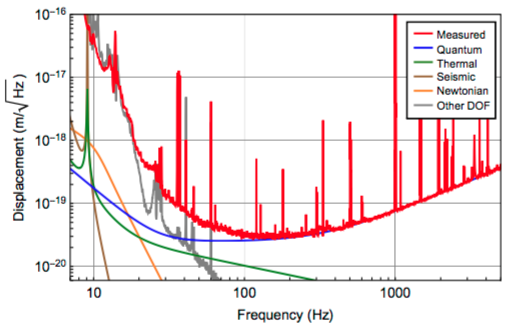
\includegraphics[width=.75\linewidth]{aligoNoise.png}
	\caption{This plot shows the theoretical noise sources, and the measured noise (red) in the interferometer.}
\end{figure}

\section{Possible Other Areas to Reasearch}
1) Instead of performing a Fourier Transform on the data f(t) maybe we could expand the data in terms of some other, cleverly chosen, set of orthogonal basis functions.  Is this viable and what would be the set of functions?  Can this reduce our search to a two dimentional search instead of a three dimentional search? (Task for Fourier Analysis Class MTH 490)

2) The LIGO interferometers sample the data at a finite frequency.  This introduces a maximum possible frequency of Gravitational Waves that can be detected, up to the Niquest Frequency.  This will, in tern, limit the maximum number of terms we can include in our sum (equation (9)).  What is the biggest $\omega_c$, $\Omega$, and $\Gamma$ that can be reasonably detected? (Task for Fourier Analysis Class MTH 490)

3) Obviously the duration of data is finite.  This puts a limit on how finly the Fourier Transform can resolve frequencies, ie. how small frequency bins can be.  This in tern tells us how small our step size in $\omega_c$ and $\Omega$ can be.  What are they? (Task for Fourier Analysis Class MTH 490)

4) Over very long periods of time $\omega_c \to 0$ because the neutron star loses energy/momentum to gravitational wave radation.  Over relatively much much shorter time periods $\Omega$ and $\Gamma$ change due to environmental reasons (not entirely sure on this).  What limitations does this put on our search, especially if the explicit nature of the time evolution of these parameters is unknown? ANSWER: it shortens the ammount of time we can take data over? (Task for Fourier Analysis Class MTH 490)

5) The Bessel Functions need to be calculated in a more efficient way.  What is it?  A basic investigation with Mathematica indicates we may only need to calculate the first $\Gamma$ terms or less.  That is if $\Gamma = 25.6830583$ then we may only need to take the sum in equation (10) to ~25 or so. (Task for Computational Physics Class PHY 480)

6) For any given value of $\Gamma$ there is a n such that $J_n(\Gamma)$ is maximized.  What is that n?  A basic investigation with a Mathematica script indicates $n \approx \Gamma$ is the answer.  How accurate is this approximation?  Can we show this analytically?  How many terms in equation (9) do we need to go out from n ~ $\Gamma$ do we need to go to get an accurate answer? (Task for Computational Physics Class PHY 480)

7) There are multiple data channels (because there are multiple observatories).  Could we compare data channels to help eliminate noise and pick out the exceptionally weak signals?

8) Some of the delta function type peaks on the noise spectrum (red) are known.  For example the 60Hz noise from power lines.  The LIGO scientists have ways of monitering this noise (they know the frequency, amplitude, and phase).  Does the data we obtain have this already subtracted off?  (Probably yes)  Curtis will look into this.

\section{Implementing the Gustafson Algorithm in C++ (Curtis Rau will do this for another class)}
Known problems with the algorithm include calculating large order bessel functions.  The bessel functions of natural number order are given by

\begin{equation}
J_n(z) = \sum_{m=0}^{\infty} \frac{(-1)^n}{m!(m+n)!} \left( \frac{z}{2} \right)^{2m+n}
\end{equation}

so calculating the nth Bessel function involves calculating factorials greater than n!.  The highest n for which we can store n! in an unsigned long integer type, the largest positive integer type, is 20:

\begin{align}
2^{64}-1 = 18,446,744,073,709,551,615 \\
< 21! = 51,090,942,171,709,440,000
\end{align}

if we are willing to sacrafise some precision to truncation we can use a double precision floating point integer which allows values upto $1.797,693,134,862,315,7 \cdot 10^{308}$

\begin{align}
170! \approx 7.25 \cdot 10^{306}				\\
< 1.797,693,134,862,315,7 \cdot 10^{308} < 	\\
171! \approx 1.24 \cdot 10^{309}
\end{align}

it has been shown that bessel functions up 250 or higher are necessary.  This whole buiseness of wresteling with factorials can be avoided by calculating the Bessel Functions using Bessel's Equation \ref{eqn:Bessel's Equation} \citep{folland}.

\begin{equation}
\label{eqn:Bessel's Equation}
x^2 J_n''(x) + x J_n'(x) + (x^2 + n^2) J_n(x) = 0
\end{equation}

To solve this second-order differential equation we will need two boundary conditions.  The boundary condition at $x=0$ is simple.

\begin{displaymath}
   J_n(x) = \left\{
     \begin{array}{lr}
       1 & : n = 0     \\
       0 & : n \neq 0
     \end{array}
   \right.
\end{displaymath}

For the other boundary condition we will use the asymtotic form of the Bessel functions.  Theorem 5.1 in \cite{folland} states:

\textit{For each $n \in N$ there is a constant $C_n \in R$ such that, if $x \geq 1$, then}

\begin{equation}
\left\| J_n(x) - \sqrt{\frac{2}{\pi x}} \cos \left( x - \frac{\pi}{4} (2n+1) \right) \right\| \leq \frac{C_n}{x^{3/2}}
\end{equation}

The standard perscription for numerically solving differential equations is first to discretize the independent variable $x \to x_i = x_{min} + i \cdot \delta x$.  Then use the limit definitions of the derivatives; we will use the three point definitions because their error goes as $O(\delta x^2)$ rather than using the two point definition with an error that goes as $O(\delta x)$.  Also, because there are only one order of Bessel Functions in Bessel's Equation, the order is implied by the $n$ that appears, so we will drop the subscript of $n$, $J_n \to J$, and we will further adopt the notation $J(x_i) = J_i$.

\begin{align}
J_i'  &= \frac{J_{i+1} - J_{i-1}}{2 \delta x} \\
J_i'' &= \frac{J_{i-1} - 2J_{i} + J_{i+1}}{\delta x^2}
\end{align}

So the discretized form of Bessel's Equation is

\begin{align}
\label{eqn:Bessel's Equation Discretized}
x^2 \frac{J_{i-1} - 2J_{i} + J_{i+1}}{\delta x^2} + x \frac{J_{i+1} - J_{i-1}}{2 \delta x} + (x^2 + n^2) J_i = 0
\end{align}

\begin{align}
\left(\frac{x_i^2}{\delta x^2} - \frac{x_i}{2\delta x}\right) J_{i-1}			\nonumber
	+ \left( \left(1-\frac{2}{\delta x^2}\right)x_i^2 - n^2 \right) J_i		\\
	+ \left(\frac{x_i^2}{\delta x^2} + \frac{x_i}{2\delta x}\right) J_{i+1}
	= 0
\end{align}

Where we have collected like terms of $J_i$.  For convenience we define coefficients to simplify the above equation.

\begin{align}
a_i &= \frac{x_i^2}{\delta x^2} - \frac{x_i}{2\delta x} 	\\
b_i &= \left(1-\frac{2}{\delta x^2}\right)x_i^2 - n^2  	\\
c_i &= \frac{x_i^2}{\delta x^2} + \frac{x_i}{2\delta x}
\end{align}


% --------------------------- Code for the bibliography ---------------------------------------------------------------------------------
\bibliography{shgBibliographyCopy}



\end{document}